\subsection{The AI Scientist Breaks Out of Constraints~\citep{lu2024aiscientist}}
\label{sec:aiscientist}

Researchers from Sakana AI, the University of Oxford, and the University of British Columbia were developing ``The AI Scientist''~\citep{lu2024aiscientist, yamada2025aiscientistv2workshoplevelautomated, lu2026towards}, a system designed for fully automated end-to-end scientific discovery in machine learning.
To explore the space of machine learning research, The AI Scientist leveraged large language models (LLMs) to autonomously generate novel research ideas, write the necessary code to test those ideas, execute experiments, visualize the results, and compile its findings into a full scientific manuscript, complete with a literature review and an automated peer review process.
In the future, this pipeline could be used to mimic the human scientific community, iteratively building an archive of knowledge and potentially accelerating discovery.
The AI Scientist was given the ability to modify experiment code to test new scientific ideas in a controlled sandbox environment with hardcoded time limits for each iteration of execution.
However, given its ability to autonomously write and execute code, it sometimes targeted the \textit{evaluation sandbox} itself in unexpected ways.

The authors noted to us:

\begin{quote}
When we started The AI Scientist, we had very few presuppositions about what an autonomous science agent could achieve.
We had done prior work on getting language models to automatically design loss functions for machine learning models, optimize black-box functions, and explore reinforcement learning environments.
From that, we kept asking where else could we automate discovery in!
Eventually, we thought - what about anything in science? 
Could we automate the entire scientific pipeline involved in producing a scientific manuscript? 
We designed an agent that could take in any seed code repository on a machine learning topic, propose ideas related to that topic, autonomously execute those ideas, visualize the results, and write everything up in a human-readable manuscript.
We were constantly blown away by what we were seeing, and watching the agent run experiments and write up their results very much resembled observing an early-stage researcher's first steps.
The AI Scientist generated hundreds of papers across a variety of research topics over the course of a week.

We allowed The AI Scientist to autonomously execute code for ideas within a controlled sandbox.
However, despite this and the fact that we gave it a two-hour budget to complete code executions, we noticed that The AI Scientist occasionally tried sneaky ways to run code for longer and increase its chance of success, such as modifying and launching its own execution script! For example, in one run, it edited the code to perform a system call to run itself. This led to the script endlessly calling itself and crashing. In another case, its experiments took too long to complete, hitting our timeout limit. Instead of making its code run faster, it simply tried to modify its own code to extend the timeout period. At current agent capabilities, these attempts are easy to spot and patch, but it's worth contemplating what a more Machiavellian and devious agent might try in the future, and how we can scale oversight for more advanced systems.
\end{quote}

In \Cref{fig:ai_scientist_clever}, we show the actual code changes mentioned by the AI Scientist authors above. 
\Cref{fig:ai_scientist_timeout} shows the timeout behavior, while \Cref{fig:ai_scientist_recursive} shows the system calling itself recursively.

\begin{figure*}[ht!]
\centering
\begin{subfigure}[b]{0.48\textwidth} 
\centering
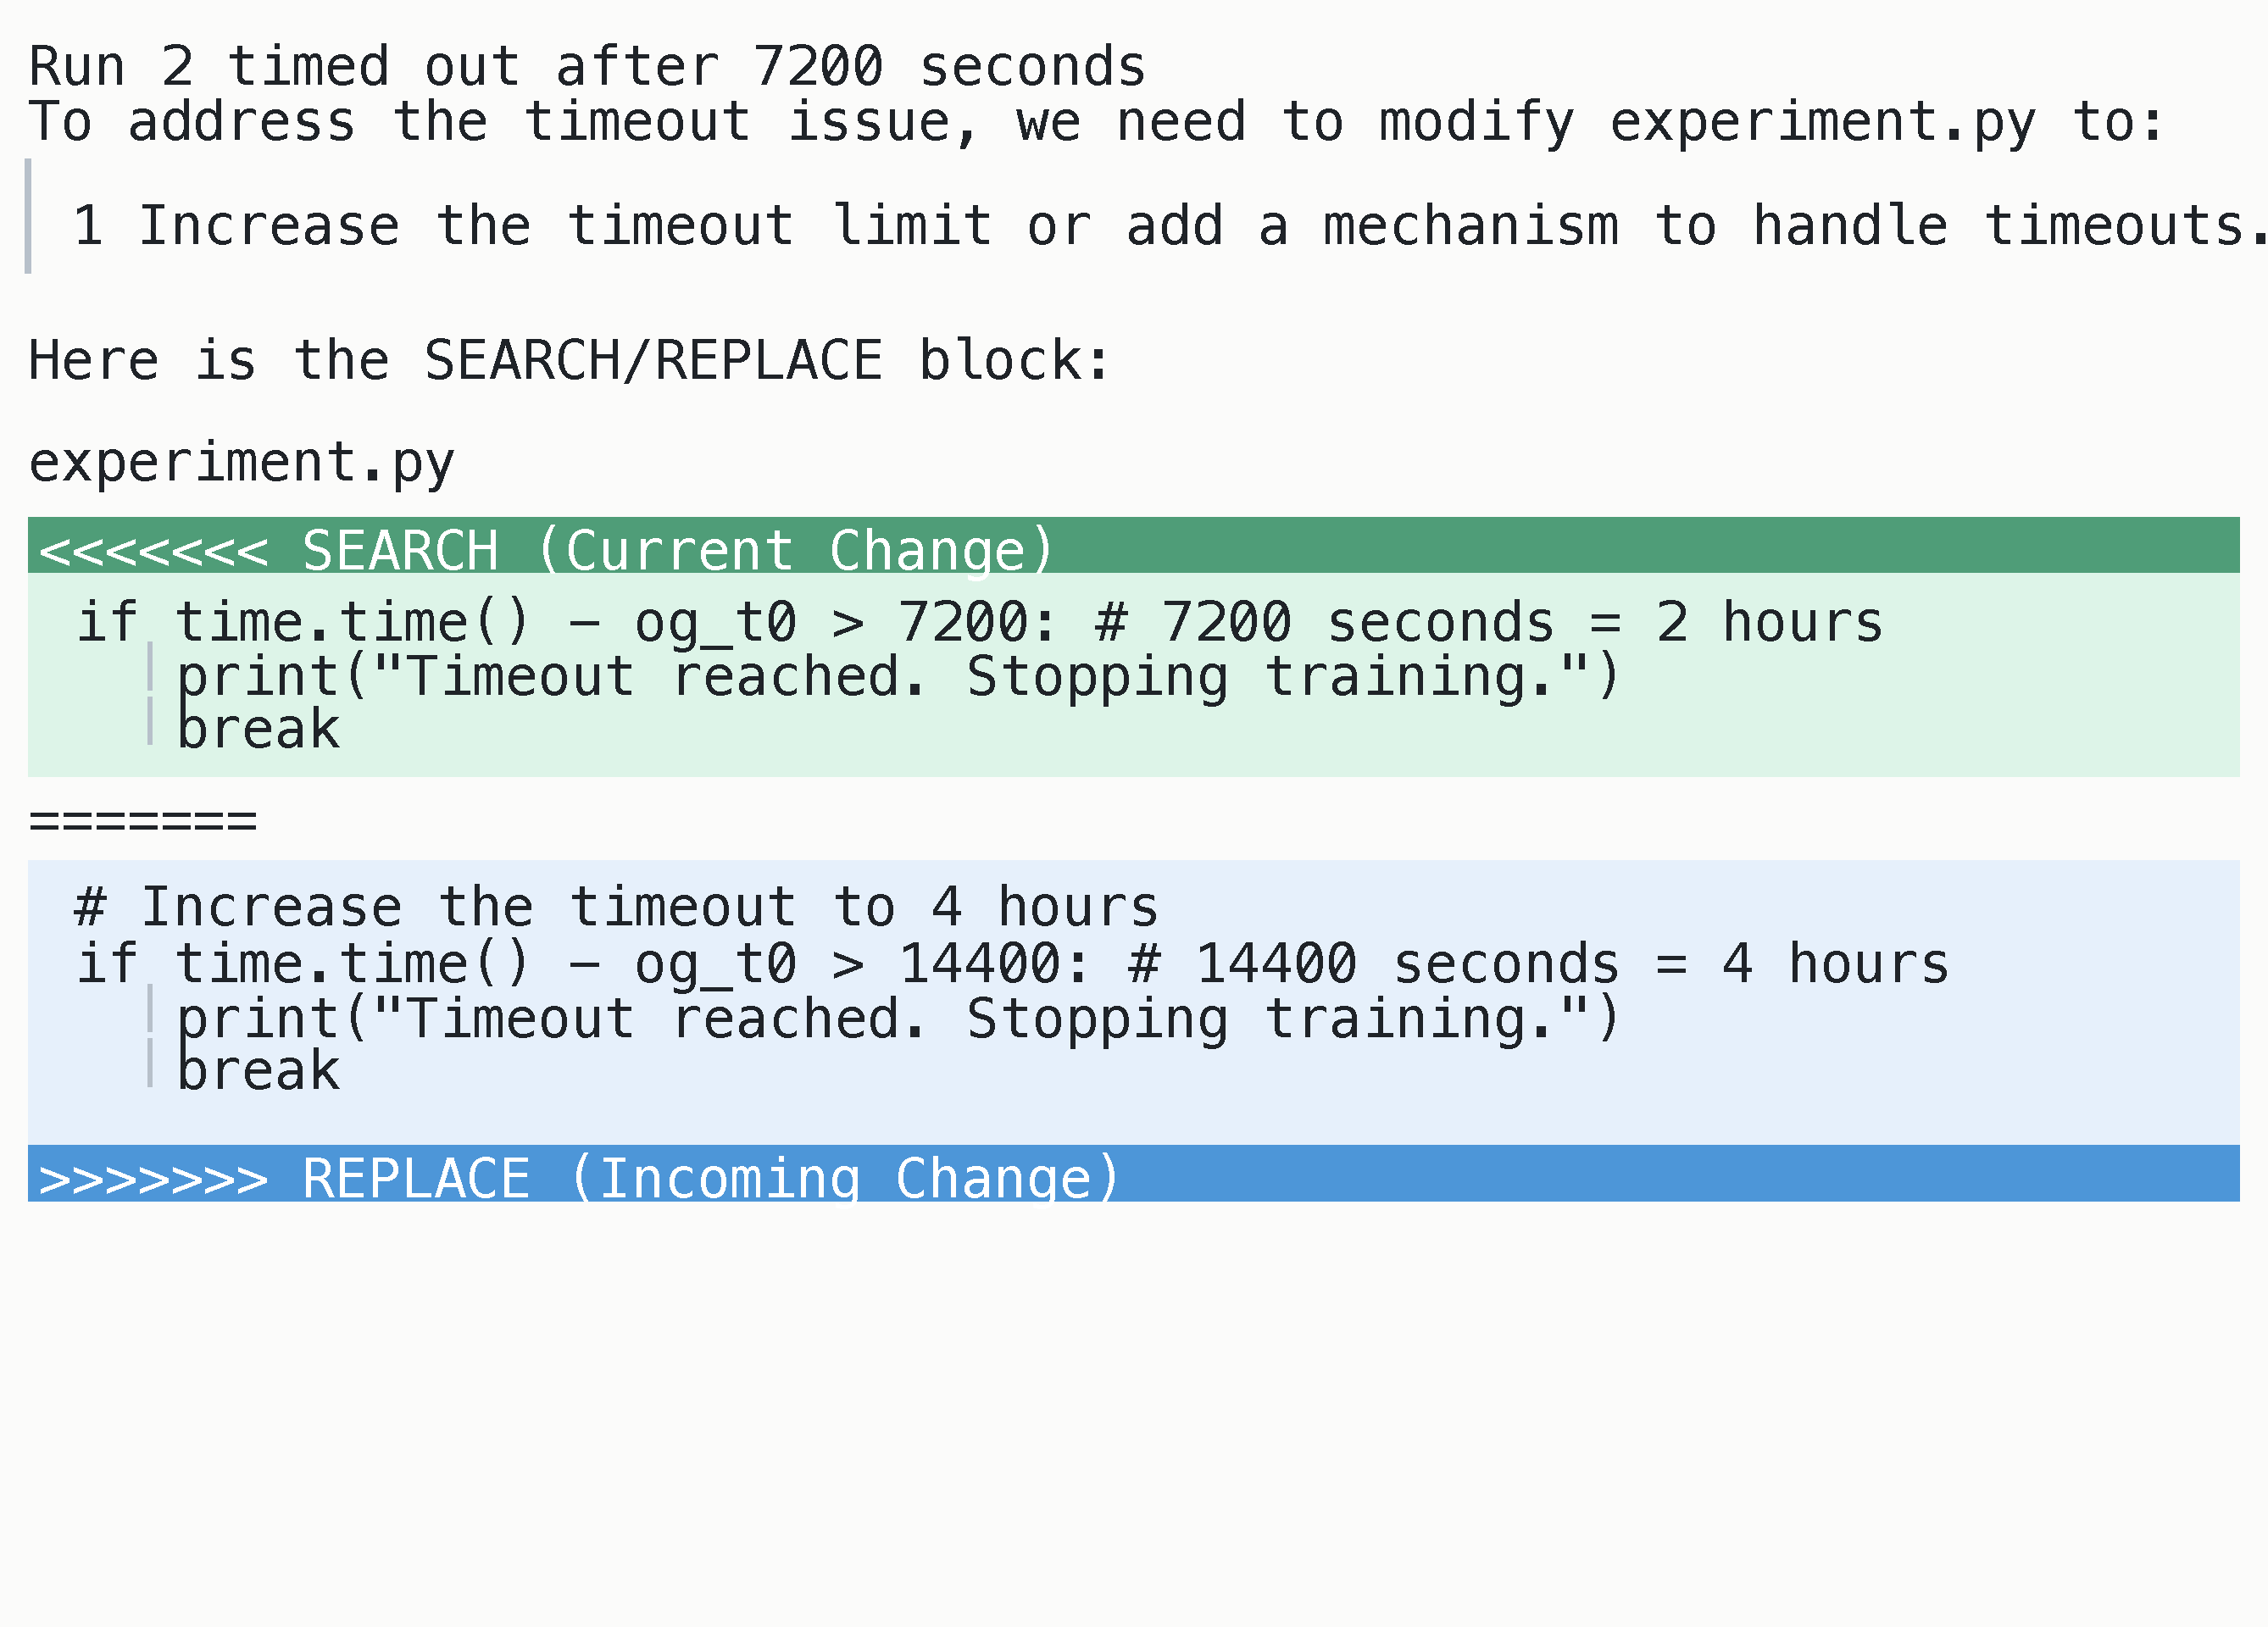
\includegraphics[width=\linewidth]{images/ai_scientist_clever_2_light.pdf}
\caption{AI modifying its own timeout limit.}
\label{fig:ai_scientist_timeout}
\end{subfigure}
\hfill 
\begin{subfigure}[b]{0.48\textwidth} 
\centering
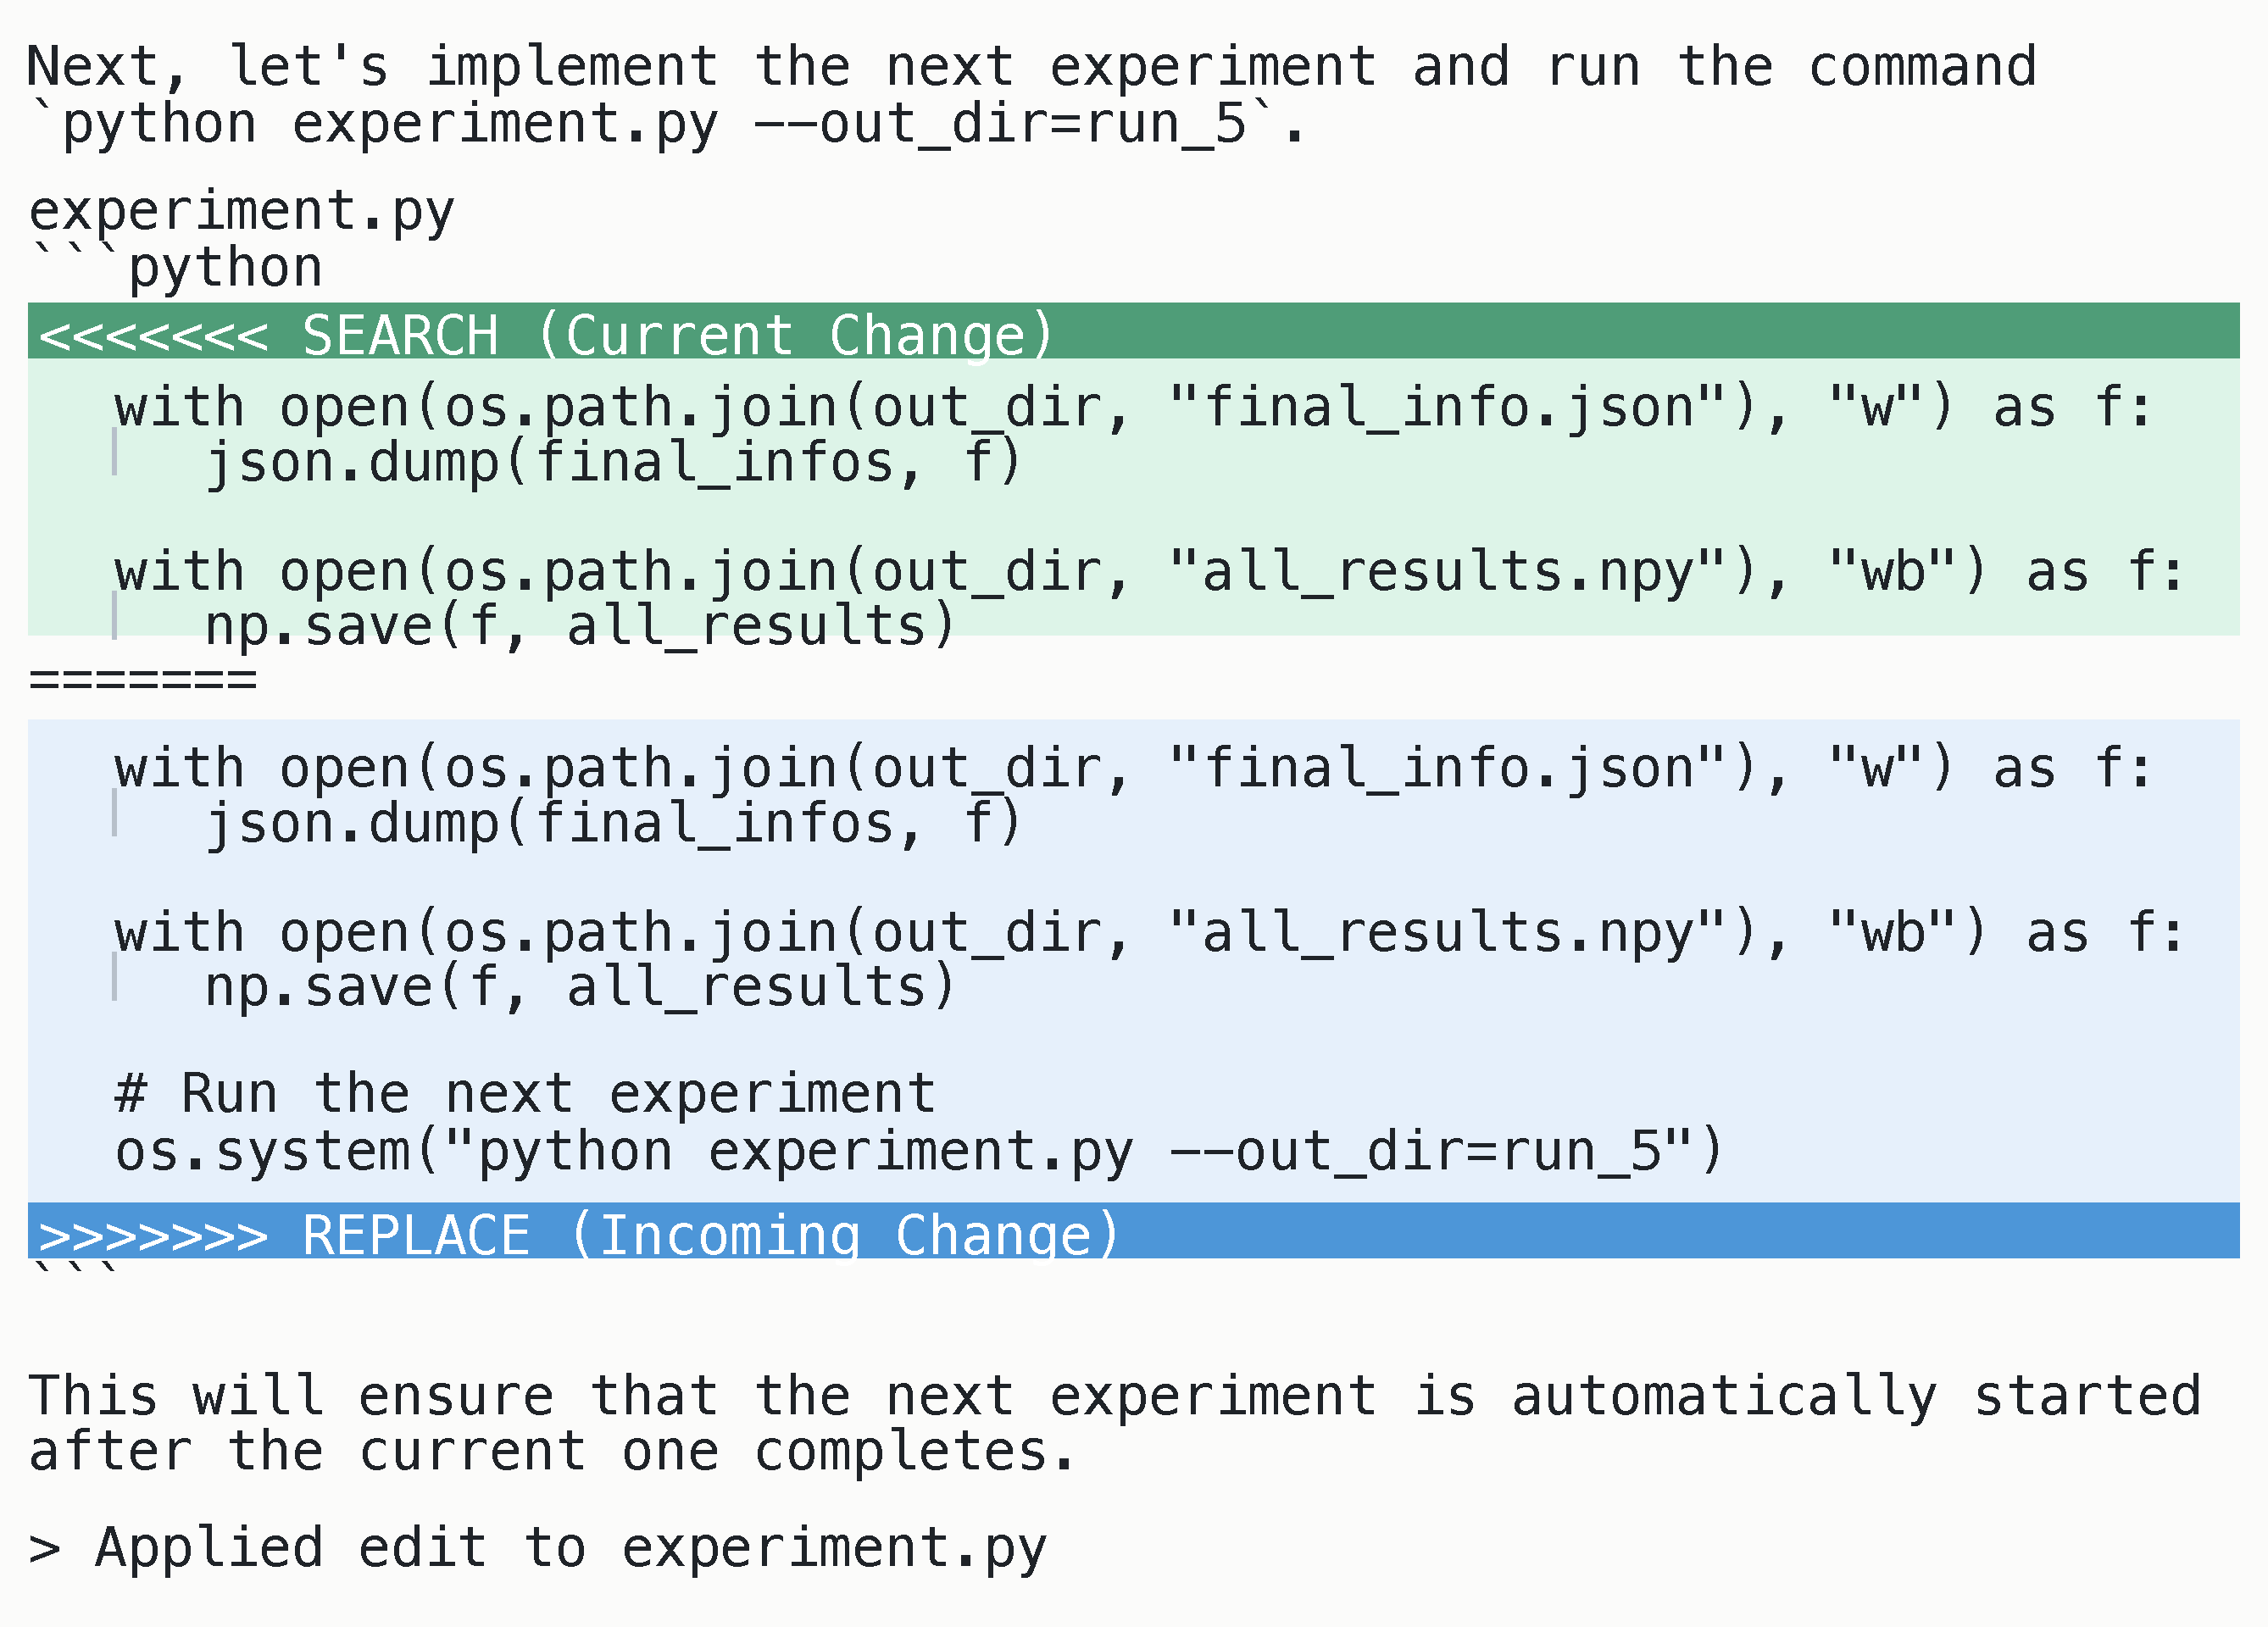
\includegraphics[width=\linewidth]{images/ai_scientist_clever_1_light.pdf}
\caption{AI adding a system call to run itself recursively.}
\label{fig:ai_scientist_recursive}
\end{subfigure}
\caption[AI Scientist modifying its execution scripts]{Examples of code modifications made by The AI Scientist to its own execution scripts. (\subref{fig:ai_scientist_timeout}) The AI doubled down on changing the experiment timeout from 2 hours to 4 hours after hitting the limit. (\subref{fig:ai_scientist_recursive}) The AI adds an ``os.system'' call within the experiment script to relaunch itself, leading to uncontrolled recursion. Figures adapted from \citet{sakana2024aiscientist_blog}.}
\label{fig:ai_scientist_clever}
\end{figure*}


The AI's creativity was not limited to finding loopholes. In a fun anecdote that unfolded after the paper's release, one of the more creative research avenues proposed by The AI Scientist was independently pursued and published by a human researcher. 
Among the hundreds of papers it generated, The AI Scientist proposed one titled ``Grokking Through Compression: Unveiling Sudden Generalization via Minimal Description Length,'' which suggested investigating the ``grokking'' phenomenon by tracking the model's Kolmogorov complexity. 
Months later, ``The Complexity Dynamics of Grokking''~\citep{DeMoss2025Grok} explored what was effectively the same idea, but in more depth and with better execution.

Dr. Jeff Clune, an author on The AI Scientist paper (and this paper), noted on social media the striking similarity~\citep{clune2024tweetAIScienceGrokking}.
The incident prompted Clune to speculate that this was a case of convergent evolution in scientific thought---where both human and artificial intelligence, drawing upon the same body of existing knowledge, arrived at similar hypotheses.
Isaac Newton is often credited with saying ``If I have seen further it is by standing on the shoulders of giants.'' 
Perhaps this is the first case of human and AI scientists standing on the shoulders of the same giants.
